\documentclass[problems]{esg8022pset} 
\usepackage{amsmath}
\usepackage{amssymb}
\usepackage{enumerate}
\usepackage{graphicx}
\usepackage{hyperref}
\usepackage{mathtools}
%\usepackage[per-mode=symbol]{siunitx} %If this line is giving you trouble, try replacing per-mode with per
%use inter-unit-separator={}\cdot{} ?
\providecommand{\uvec}[1]{{\hat{\bf{#1}}}}
%\usepackage{pgf,tikz}
%\usetikzlibrary{arrows}
\usepackage{wasysym}
\usepackage{subfig}
\makeatletter
\newcommand{\interitemtext}[1]{%
  \begin{list}{}
   {\itemindent=0mm\labelsep=0mm
   \labelwidth=0mm\leftmargin=0mm
   \addtolength{\leftmargin}{-\@totalleftmargin}}
    \item #1
  \end{list}
}
\makeatother
\renewcommand{\d}{\,d}
\providecommand{\norm}[1]{\lVert#1\rVert}

\AtBeginDocument{%
  % Appologies to any future editor on the inconsistencies in TeX code and the unnecessary braces.  I'm aggregating previously typeset problems, and didn't think it worth my time to improve the quality of TeX code in ways that won't make any difference to the typeset material. -Jason Gross (jgross@mit.edu)
}%
\classname{Physics 8.022} \semester{Spring 2011} 
\problemsetnumber{10}
\date{\today }
\duedate{Wednesday, April 27th, 10 pm}
\readingassignment{}
\problemsettitle{RLC circuits, AC circuits}
\begin{document}
\section{Problem \thesection: Purcell 7.17}
  In the circuit shown in the diagram the 10-volt battery has negligible
  internal resistance.  The switch $S$ is closed for several seconds, then
  opened.  Make a graph with the potential of point $A$ with respect to
  ground, just before and then for 10 milliseconds after the opening of
  switch $S$.  Show also the variation of the potential at point $B$ in the
  same period of time.

  \begin{center}
    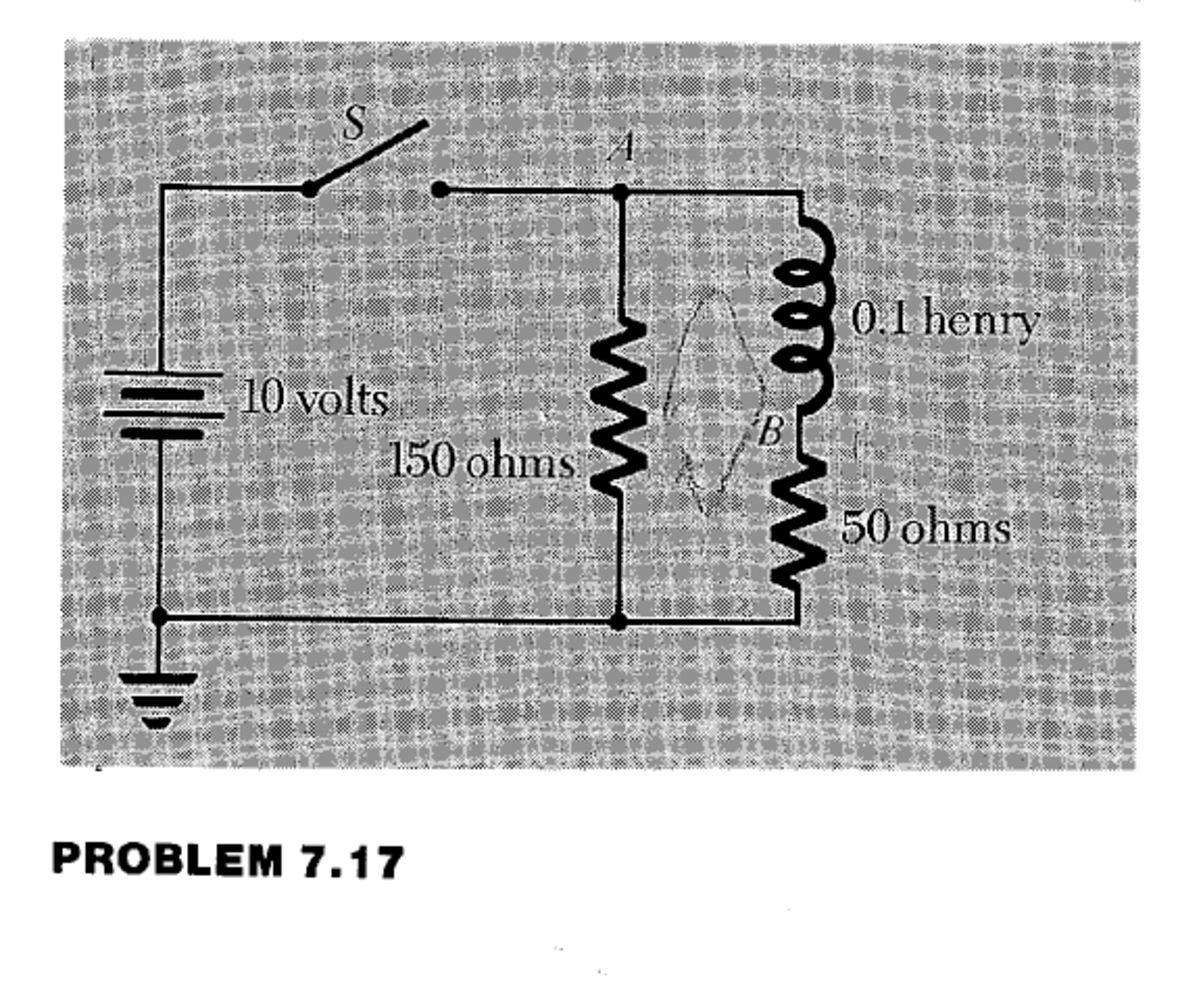
\includegraphics[width = 0.6\textwidth]{figpu717}
  \end{center}

  Extra question --- By grounding this circuit, we make the switch
  safer to operate. Describe why a large spark jumps across the switch
  when it is not grounded, and why the spark does not happen when it is
  grounded.
\section{Problem \thesection: Purcell 8.4}
  In the resonant circuit shown in the figure below, the dissipative
  element is a resistor $R'$ connected in parallel rather than in series,
  with the $LC$ combination.  Work out the equation analogous to Equation 2
  in Purcell,
  \begin{equation*}
    \frac{d^2V}{dt^2} + \left(\frac{R}{L}\right)\frac{dV}{dt} + \left(\frac{1}{LC}\right)V = 0,
  \end{equation*}
  which applies to this circuit.  Find also the conditions on the solution
  analogous to those that hold in the series $RLC$ circuit.  If a series
  $RLC$ and a parallel $R'LC$ circuit have the same $L$, $C$, and $Q$
  (quality factor), how must $R'$ be related to $R$?

  \begin{center}
    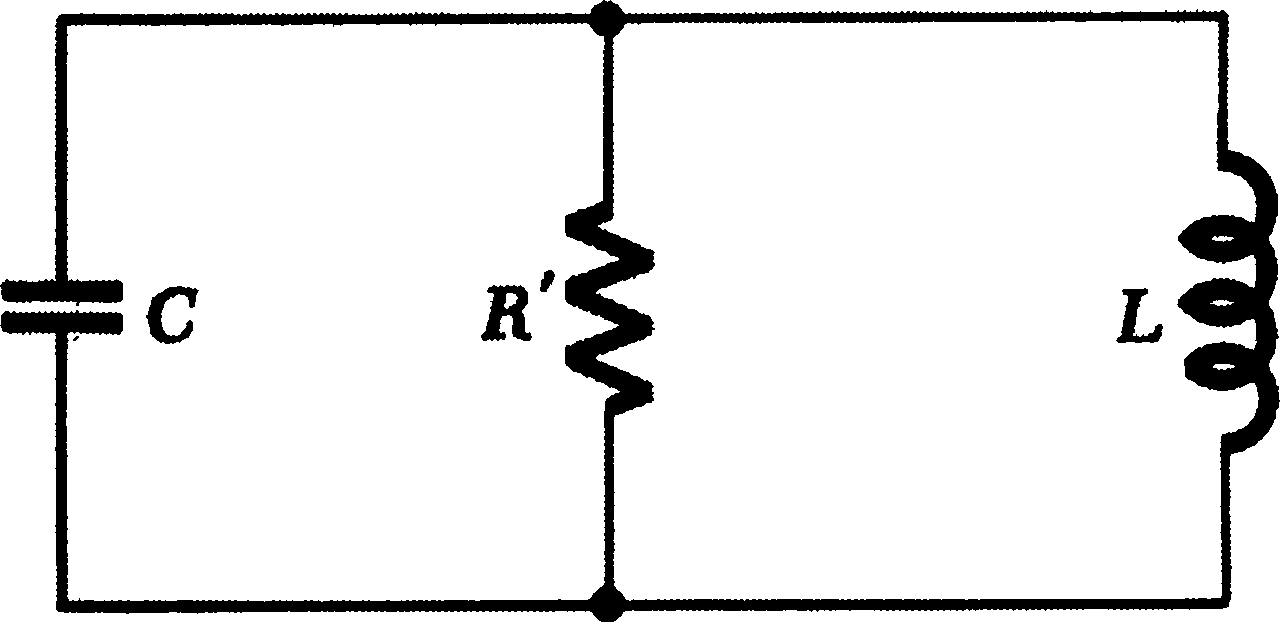
\includegraphics[width = 0.6\textwidth]{figpu804}
  \end{center}
\section{Problem \thesection: Purcell 8.7}
  A resonant cavity of the form illustrated is an essential part of many
  microwave oscillators. It can be regarded as a simple $LC$ circuit. The
  inductance is that of a toroid with one turn. Find an expression for the
  resonant frequency of this circuit and show by a sketch the configuration
  of the magnetic and electric fields.
  Hint: the capacitor is composed by the upper and lower disks
  \begin{center}
    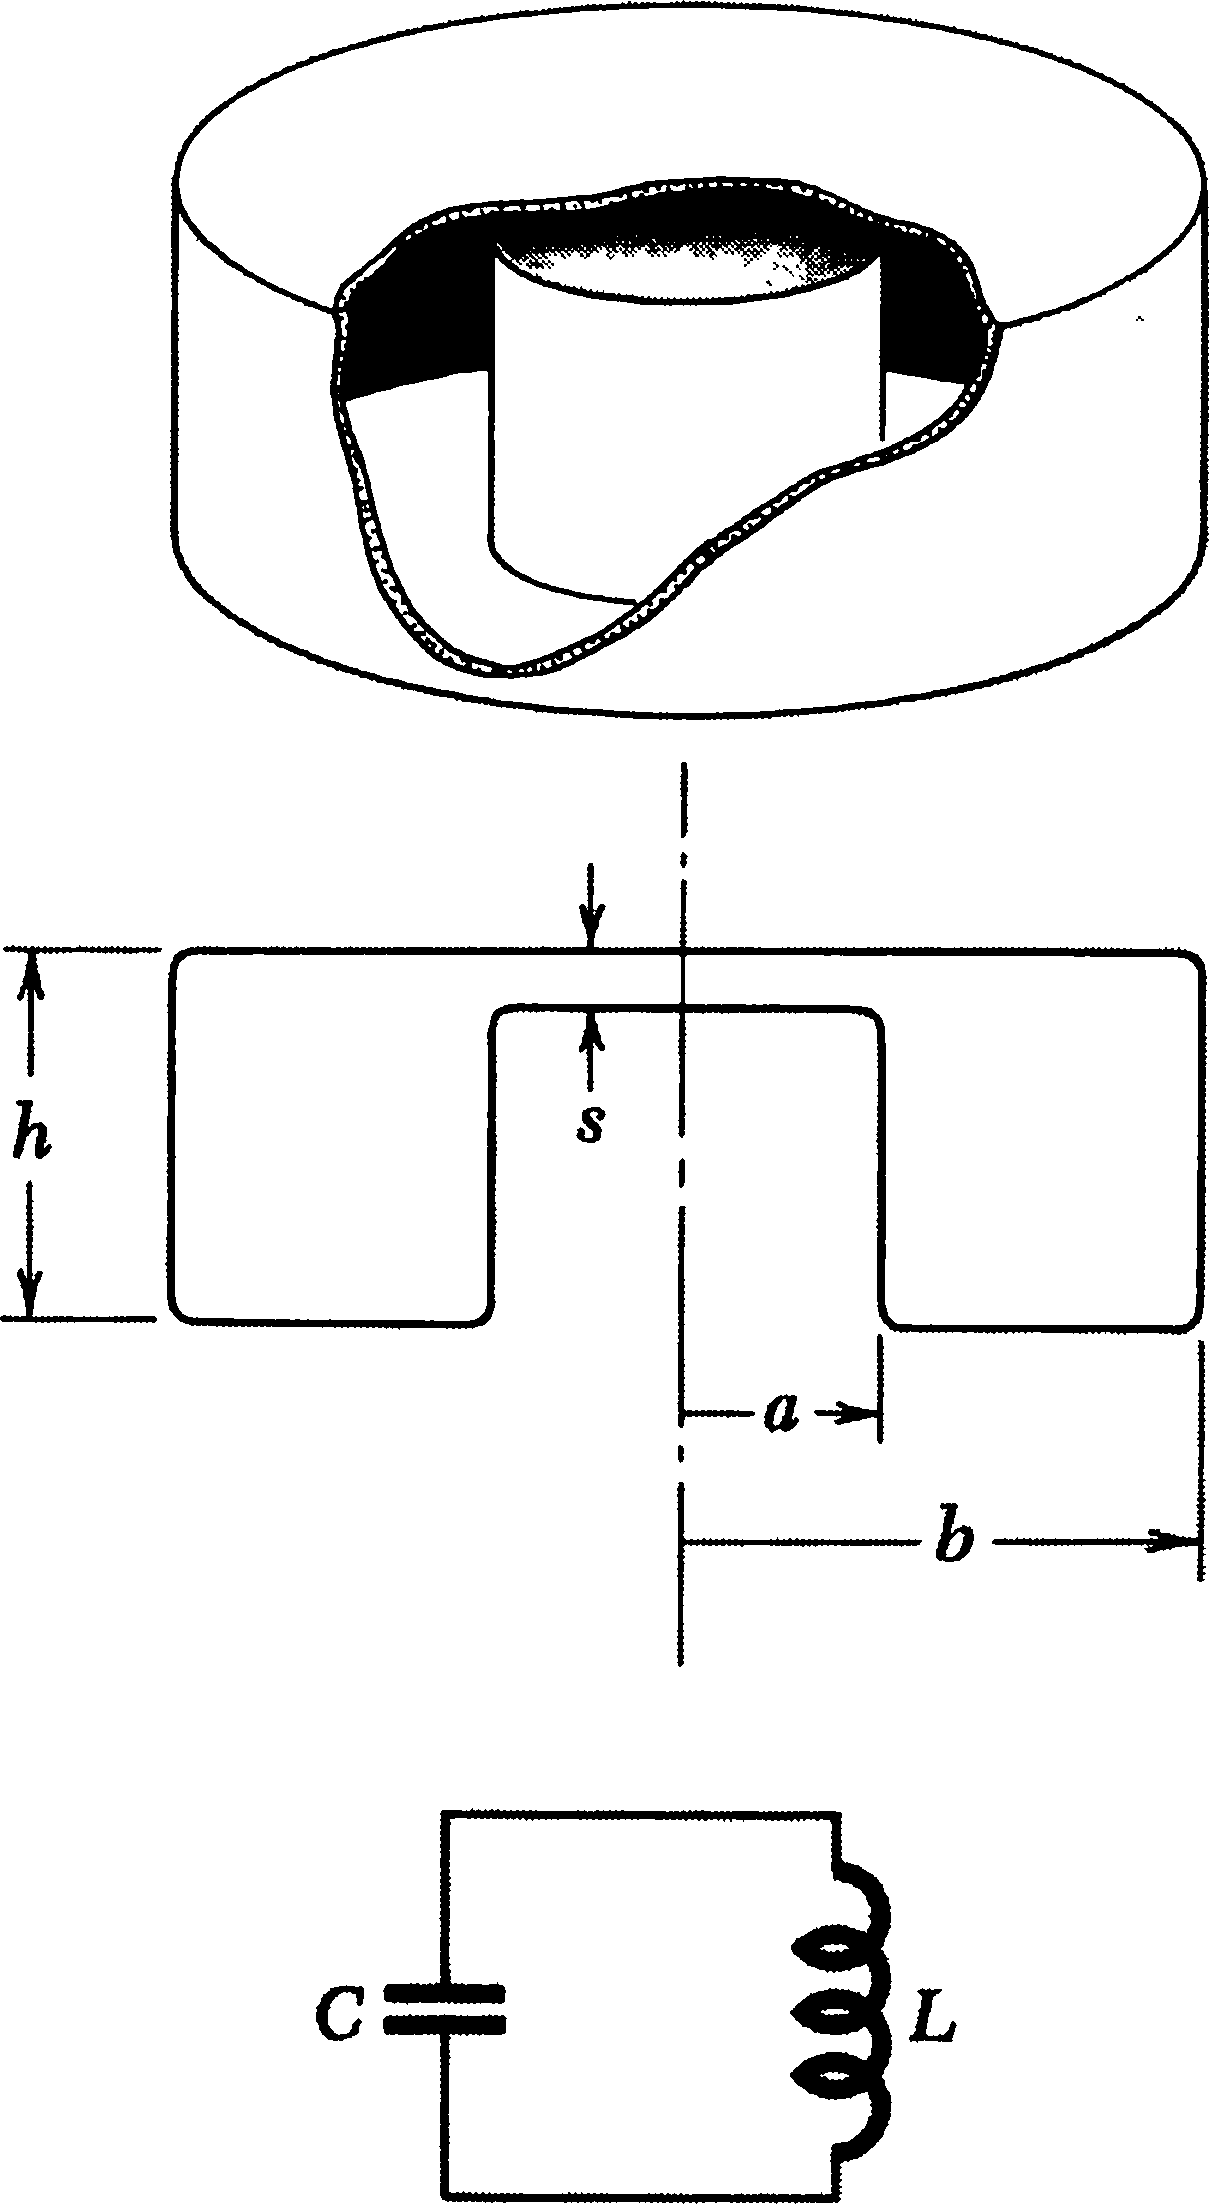
\includegraphics[width = 4cm]{pu807}
  \end{center}
\section{Problem \thesection: Purcell 8.9}
  Using the equations 10 and 13 in Purcell (below), express the effect of
  damping on the frequency of a series $RLC$ circuit.
  \begin{equation*}
    \omega^2 = \frac{1}{LC} - \alpha\frac{R}{L} + \alpha^2 = \frac{1}{LC} - \frac{R^2}{L^2}
  \end{equation*}
  \begin{equation*}
    Q = \omega \frac{\text{energy stored}}{\text{average power dissipated}}
  \end{equation*}
  Let $\omega_0 = 1 / \sqrt{LC}$ be the frequency of the undamped circuit.
  Suppose enough resistance is added to bring $Q$ from $\infty$ down to
  1000.  By what percentage is the frequency $\omega$ thereby shifted from
  $\omega_0$?

  \begin{center}
    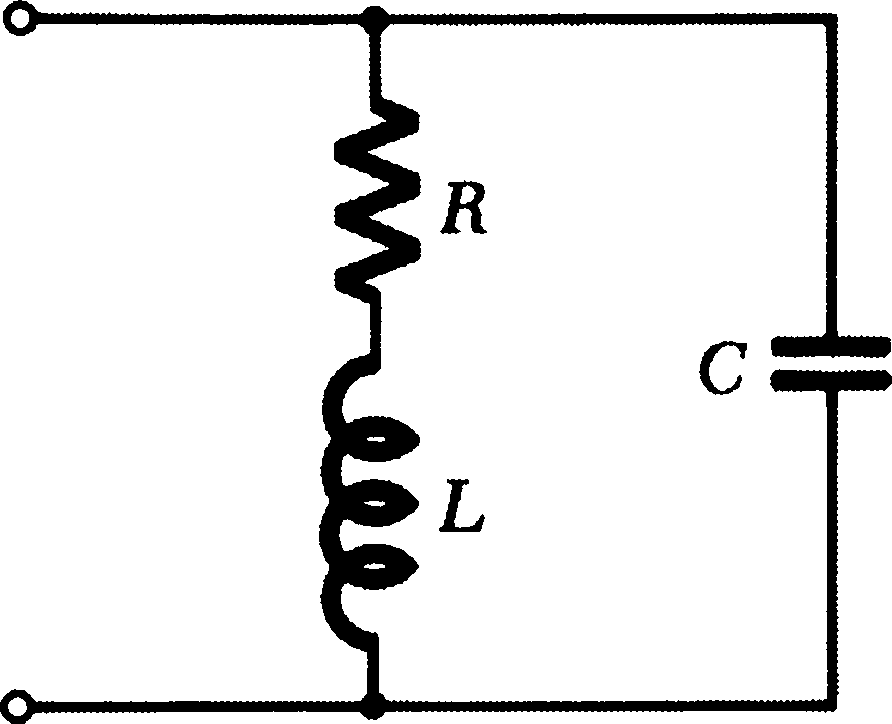
\includegraphics[width = 0.5\textwidth]{figpu809}
  \end{center}
\section{Problem \thesection: Purcell 8.12}
  Let $V_{AB} = V_B - V_A$, in this circuit.  Show that $|V_{AB}|^2 =
  V_0^2$ for any frequency $\omega$.  Find the frequency for which $V_{AB}$
  is $90^\circ$ out of phase with $V_0$.

  \begin{center}
    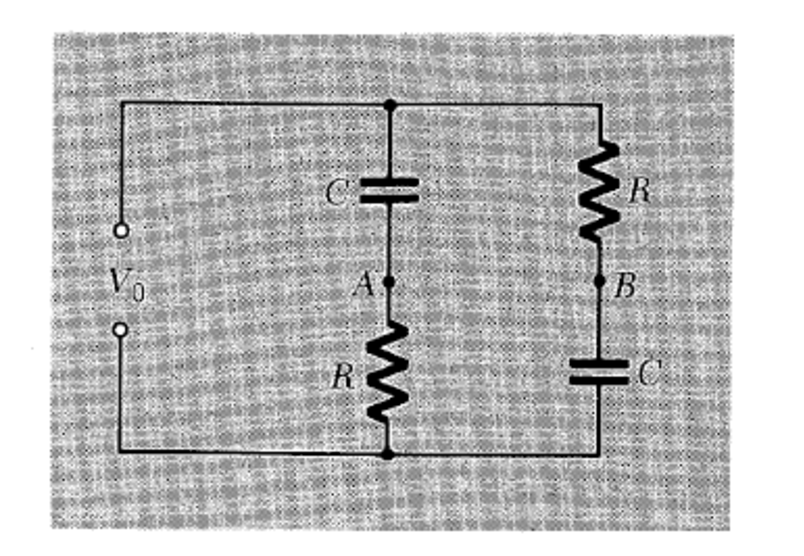
\includegraphics[width = 0.5\textwidth]{figpu812}
  \end{center}
\section{Problem \thesection: Purcell 8.16}
  \begin{center}
    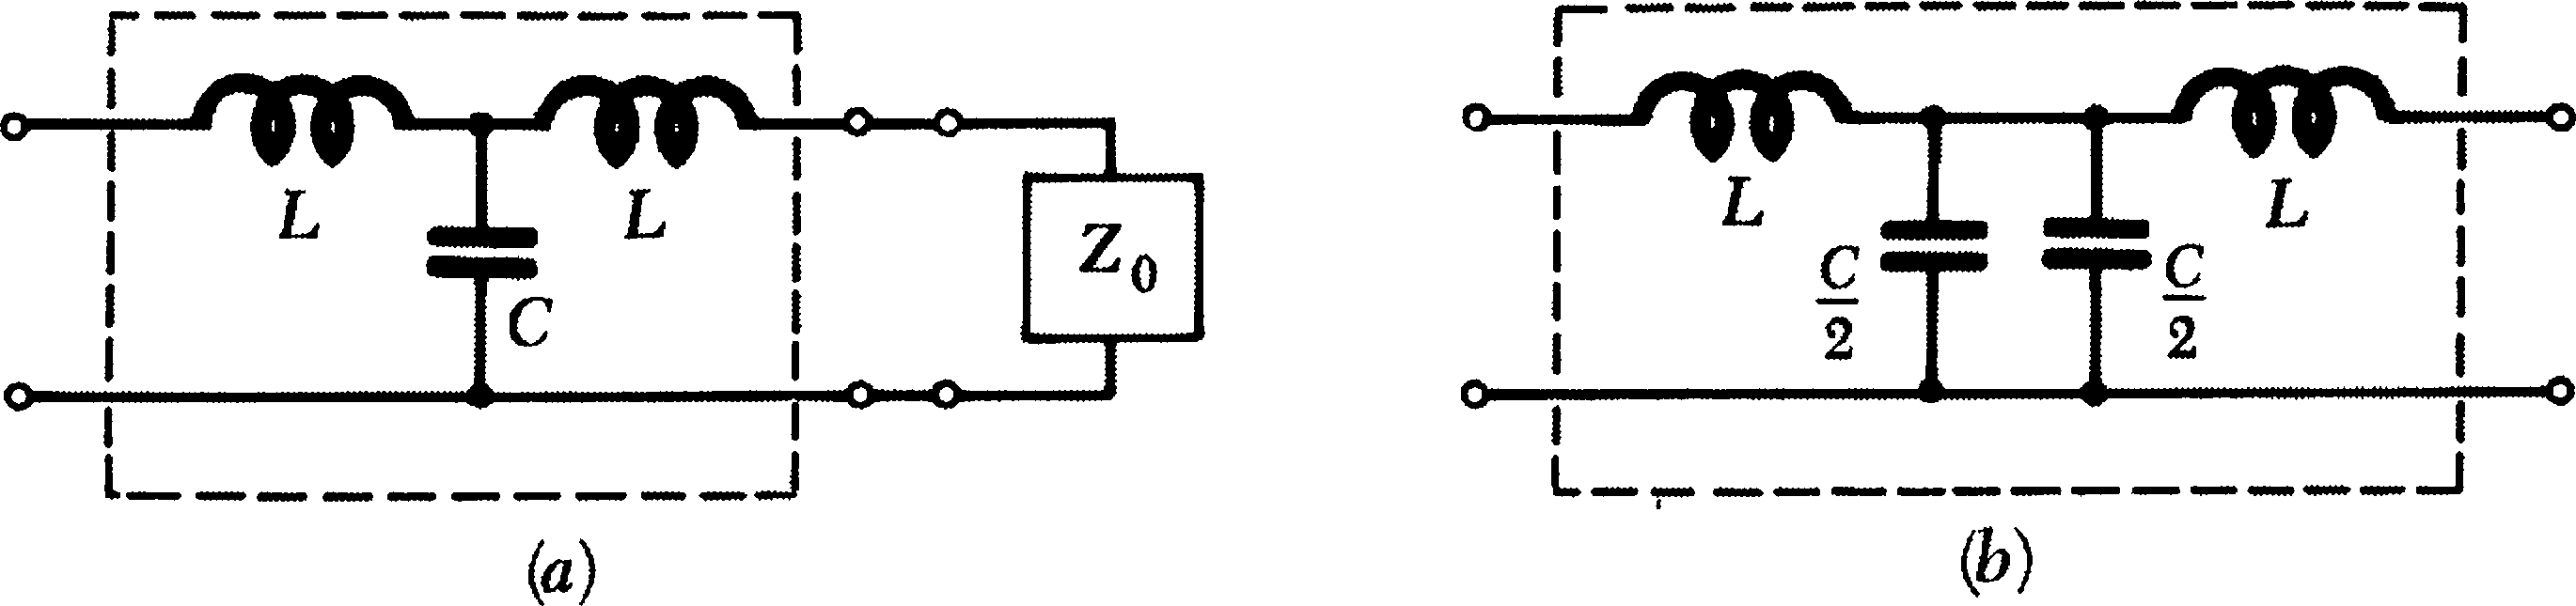
\includegraphics[width = 0.75\textwidth]{pu816}
  \end{center}

  \noindent The box (a) with four terminals contains a capacitor $C$ and
  two inductors of equal inductance $L$ connected as shown.  An impedance
  $Z_0$ is to be connected to the terminals on the right. For a given
  frequency $\omega$ find the value which $Z_0$ must have if the resulting
  impedance across the left terminals is $Z_0$. You will find that the
  required $Z_0$ is a pure resistance $R_0$ provided $\omega^2<2/LC$. What
  is $Z_0$ in the special case $\omega = \sqrt{2/LC}$?  It helps in
  understanding that case to note that the contents of the box (a) can be
  equally well represented by box (b).
\section{Problem \thesection: Optional Purcell 8.10}
  Is it possible to find a frequency at which the impedance at the
  terminals of the circuit below will be purely real?

  \begin{center}
    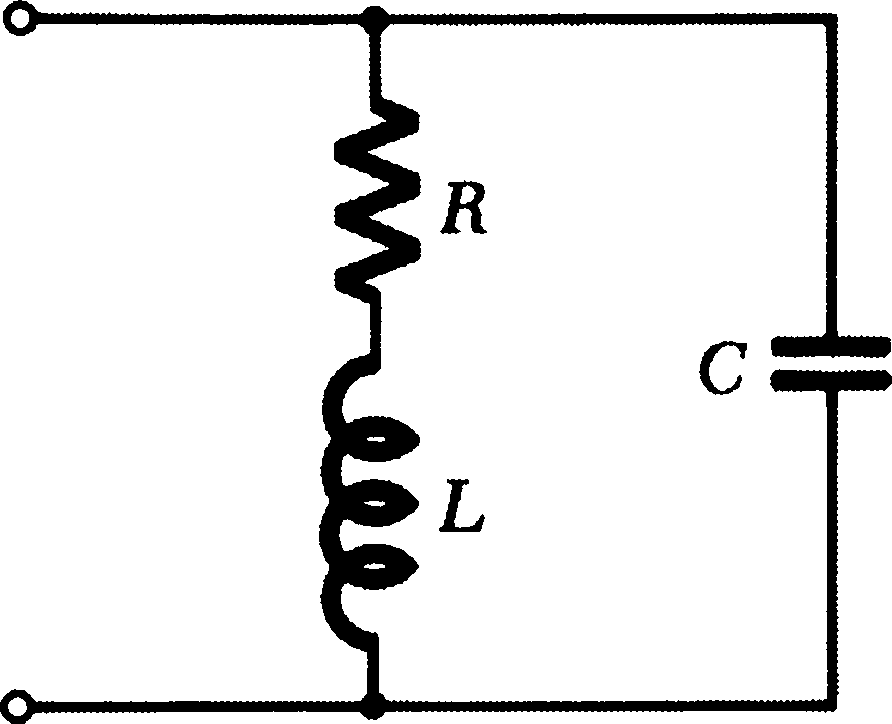
\includegraphics[width = 0.5\textwidth]{figpu810}
  \end{center}
\section{Problem \thesection: Optional Purcell 8.13}
  Show that, if the condition $R_1R_2 = L / C$ is satisfied by the
  components of the circuit below, the difference in voltage between points
  $A$ and $B$ will be zero at any frequency.  Discuss the suitability of
  this circuit as an AC bridge for measurement of an unknown inductance.

  \begin{center}
    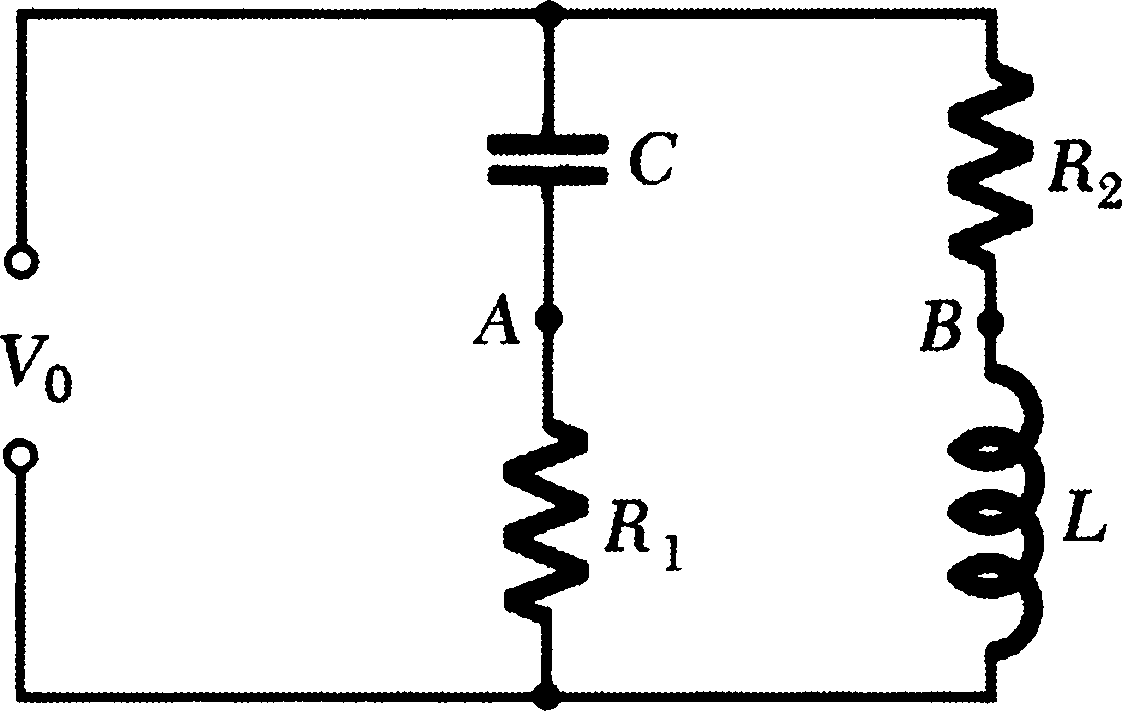
\includegraphics[width = 0.5\textwidth]{figpu813}
  \end{center}
\section{Problem \thesection: Optional Purcell 8.14}
  In the laboratory, you find an inductor of unknown inductance $L$ and
  unknown internal resistance $R$.  Using a DC ohm-meter, an AC volt-meter
  of high impedance, a 1-microfarad capacitor, and a 1000-Hz signal
  generator, determine $L$ and $R$ as follows: According to the ohm-meter,
  $R$ is 35 ohms.  You connect the capacitor in series with the inductor
  and the signal generator.  The voltage across both is 10.1 volts.  The
  voltage across the capacitor alone is 15.5 volts. You note also, as a
  check, that the voltage across the inductor alone is 25.4 volts.  How
  large is $L$?  Is the check consistent?
\end{document}
